\documentclass{beamer}
\usetheme{default}
\usecolortheme{crane}
\usepackage{amsmath}
\usepackage{amsfonts}
\usepackage{epstopdf}
\usepackage{amssymb}
\usepackage{graphicx}
\usepackage{movie15}
\newcommand\scalemath[2]{\scalebox{#1}{\mbox{\ensuremath{\displaystyle #2}}}} % for scaling math
%\usepackage{CJKutf8}
\title{OpenLCDFDM: an finite-difference LCD simulator}
\author{\texorpdfstring{Zong-han, Xie\newline\url{icbm0926@gmail.com}}{Zong-han, Xie}}
\date{\today}
\begin{document}
%\begin{CJK}{UTF8}{cwmc}
\begin{frame}
\titlepage
\end{frame}
\begin{frame}[label=licensepage]
\frametitle{License of this slide}
This slide made by Zong-han, Xie (\href{icbm0926@gmail.com}{icbm0926@gmail.com}) is licensed under Creative Commons Attribution-NonCommercial 4.0 International License. \newline
\begin{center}
\includegraphics[scale=1.0]{by-nc-sa.eps}
\end{center}
\end{frame}
\AtBeginSection[]
{
  \begin{frame}
    \frametitle{Outline}
    \tableofcontents[currentsection]
  \end{frame}
}
\begin{frame}
\frametitle{LCD on consumer products}
\begin{center}
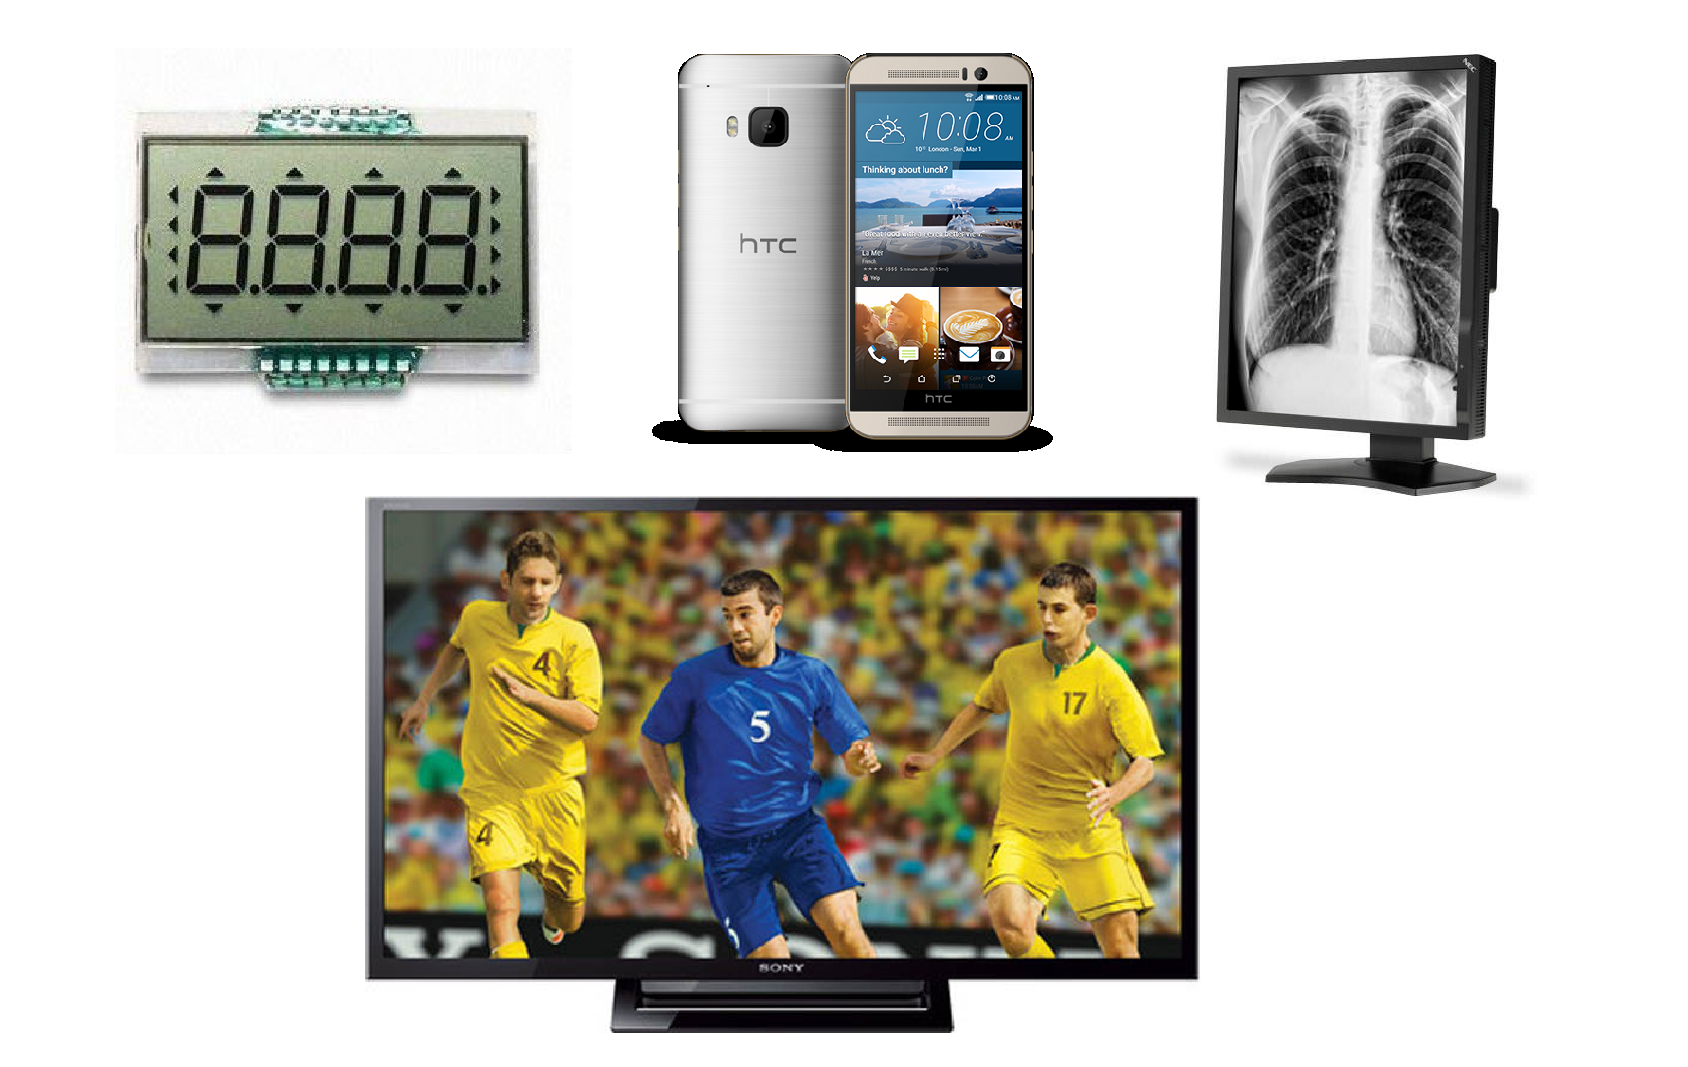
\includegraphics[scale=0.4]{LCD_Consumers.eps}
\end{center}
\end{frame}
\begin{frame}
\frametitle{LCD display structure}
\begin{center}
\includegraphics[scale=0.4]{LCD_Infografik_ENG_580_tcm1113_40163.jpg}
\\
Liquid crystal layer is served as an optical switch, it determines how much light from light source (backlight in LCD display) can propagate through.
\end{center}
\end{frame}
\begin{frame}
\frametitle{Polarization}
\begin{center}
\includegraphics[scale=0.4]{polarization.png}
\end{center}
\end{frame}
%\begin{frame}
%\frametitle{Birefringence and phase retardation}
%If a material has nonisotropic refractive index, it is called a birefringence material. It causes different light speed on different polarization. It canges phase diefference between
%two polarization of light, it's called phase retardation.
%\begin{center}
%\includegraphics[scale=0.4]{retardation.png}
%\end{center}
%\end{frame}
\begin{frame}
\frametitle{Birefringence}

\end{frame}

\begin{frame}
\frametitle{Electric controlled LC orientation}
\begin{center}
\includegraphics[scale=0.4]{ECB.jpg}
\end{center}
Due to the nonisotropic dielectric property of liquid crystal, when external electric field is applied, the LC molecule will start to align with the electric field.
\end{frame}
\begin{frame}
\frametitle{LCD operating modes}

\end{frame}
\begin{frame}
\frametitle{Calculation models}
\begin{itemize}
\item<1-> Find LC distribution:
\begin{itemize}
\item<1-> Oseen-frank free energy for liquid crystal
\item<1-> Laplace equation in nonisotropic media
\end{itemize}
\item<1-> Optical calculation: Extended Jones matrix method
\end{itemize}
\end{frame}
\begin{frame}
\frametitle{Calculate LC Orientation}
Using Oseen-frank elastic free energy density to model the elastic property of the liquid crystal layer.
The LC molecule distribution is acquired by minimizing the total energy density which includes elastic free energy density and electric field energy density.
The total energy density has the following form ~\cite{ShinTson}.
\begin{eqnarray}
f(\vec x) &=& \frac{1}{2}K_{11}(\nabla\cdot\vec n)^2+\frac{1}{2}K_{22}(\vec n\cdot\nabla\times\vec n)^2 + \frac{1}{2}K_{22}(\vec n\times\nabla\times\vec n)^2\nonumber \\
&&+q_0K_{22}(\vec n\cdot\nabla\times\vec n) - \frac{1}{2}K_{22}(\vec D\times\vec E)\nonumber
\label{eq:free_energy}
\end{eqnarray}
where $\vec D = \epsilon(\vec x)\cdot \vec E$ and $\epsilon(\vec x)$ is a 3X3 dielectric tensor. $\vec n(\vec{x})$ is a unit vector for local liquid crystal orientation.
\end{frame}
\begin{frame}
\frametitle{Calculate LC Orientation}
To calculate minimum free energy, \emph{Euler-Lagrange equation} is applied. OpenLCDFDM uses finite difference method to solve Euler-Lagrange equation of the total energy density to get liquid crysal distribution of minimized free energy.\\
The Euler-Lagrange equation of the free energy is solved through iterative method.
\begin{eqnarray}
\frac{\partial n_i}{\partial t} = \frac{1}{\gamma} \left( -\frac{\delta f}{\delta n_i} \right), i = x, y, z \\ \nonumber
\end{eqnarray}
$\gamma$ uses rotational viscosity.
\end{frame}
\begin{frame}
\frametitle{Laplace equation in nonisotropic and inhomogeneous media}
Laplace equation:
\begin{eqnarray}
\nabla \cdot \overleftrightarrow{\epsilon}(\vec x) \cdot \nabla \phi(\vec x) &=& 0 \nonumber
\label{eq:laplace}
\end{eqnarray}
$\overleftrightarrow{\epsilon}(\vec x)$ is the local dielectric tensor decided by the local oritation of LC molecule. 
\\
\begin{eqnarray}
\overleftrightarrow{\epsilon}(\vec x) = 
\scalemath{0.7}{
\begin{bmatrix}
\epsilon_{\perp}+\vartriangle\epsilon \sin^2\theta(\vec{x})\cos^2\phi(\vec{x}) & \frac{\vartriangle\epsilon}{2} sin^2\theta(\vec{x})\sin 2\phi(\vec{x}) & \frac{\vartriangle\epsilon}{2} \sin 2\theta(\vec{x})\cos\phi(\vec{x}) \\
\frac{\vartriangle\epsilon}{2} \sin^2\theta(\vec{x})\sin 2\phi(\vec{x}) & \epsilon_{\perp}+\vartriangle\epsilon \sin^2\theta(\vec{x})\sin^2\phi(\vec{x}) & \frac{\vartriangle\epsilon}{2} \sin 2\theta(\vec{x})\sin\phi(\vec{x}) \\
\frac{\vartriangle\epsilon}{2} \sin 2\theta(\vec{x})\cos\phi(\vec{x}) & \frac{\vartriangle\epsilon}{2} \sin 2\theta(\vec{x})\sin\phi(\vec{x}) & \epsilon_{\perp}+\vartriangle\epsilon \cos^2\theta(\vec{x})\\ 
\end{bmatrix}}
\nonumber
\label{eq:dielectric_tensor}
\end{eqnarray}
\\
where $\theta(\vec{x})$ and $\phi(\vec{x})$ is the local orientation of liquid crystal molecule, $\vartriangle\epsilon = \epsilon_{\parallel}-\epsilon_{\perp}$.
\end{frame}
\begin{frame}
\frametitle{Extended Jones matrix method for uniaixal media}
Under the assumption of $n_e \approxeq n_o$, the e-ray and o-ray propagate on the same direction. With this assumption, Jones matrix can be modified into extended Jones matrix method.
\begin{eqnarray}
\vec{J}_{out} = 
\scalemath{0.9}{
\begin{bmatrix}
{t'}_s & 0 \\ 0 & {t'}_p
\end{bmatrix}
\begin{bmatrix}
\vec{e}\cdot\vec{s} & \vec{o}\cdot\vec{s} \\ \vec{e}\cdot\vec{p} & \vec{o}\cdot\vec{p}
\end{bmatrix}
\begin{bmatrix}
e^{ik_e\vartriangle z} & 0 \\ 0 & e^{ik_o\vartriangle z}
\end{bmatrix}
\begin{bmatrix}
\vec{s}\cdot\vec{e} & \vec{p}\cdot\vec{e} \\ \vec{s}\cdot\vec{o} & \vec{p}\cdot\vec{o}
\end{bmatrix}
\begin{bmatrix}
t_s & 0 \\ 0 & t_p
\end{bmatrix}
}
\vec{J}_{in} \\ \nonumber
\nonumber
\label{eq:extendedJones}
\end{eqnarray}
\begin{center}
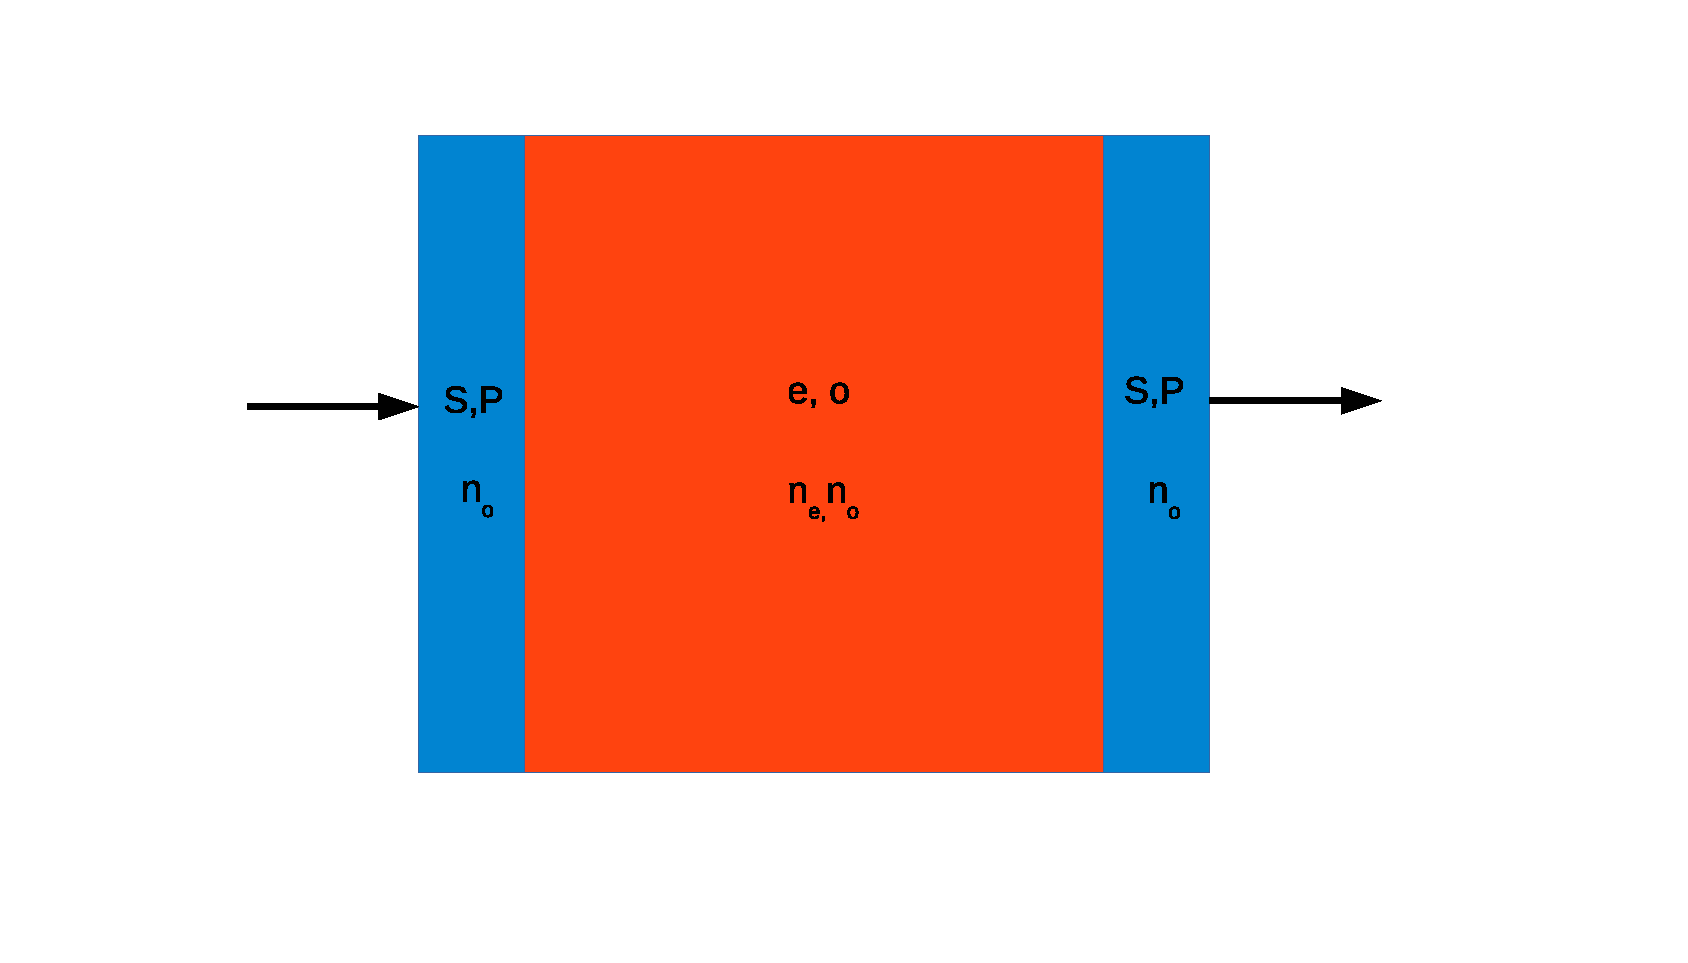
\includegraphics[scale=0.25]{extj_uniaxial.eps}
\end{center}
${t'}_s$, ${t'}_p$ ${t'}_s$ and ${t'}_p$ are transmission rate for s wave and p wave acquired through Fresnel's euations.
\end{frame}
\begin{frame}
\frametitle{Extended Jones matrix method for isotropic mediaand calculation for transmission rate}
For isotropic media, the Jones matrix only needs to calculate transmission rate for s wave and p wave.
\begin{eqnarray}
\vec{J}_{out} = 
\scalemath{0.9}{
\begin{bmatrix}
{t}_s & 0 \\ 0 & {t}_p
\end{bmatrix}
}
\vec{J}_{in} \nonumber
\nonumber
\label{eq:extendedJones_iso}
\end{eqnarray}
Transmision rate for incoherent light source:
\begin{eqnarray}
M = M_1M_2M_3... = 
\begin{bmatrix}
m_{11} & m_{12} \\ m_{21} & m_{22}
\end{bmatrix}
\nonumber
\end{eqnarray}
\begin{eqnarray}
T = 0.5*(m_{11}^2 + m_{12}^2 + m_{21}^2 + m_{22}^2) \nonumber
\end{eqnarray}
\end{frame}
\begin{frame}
\frametitle{OpenLCDFDM program structures}
\begin{center}
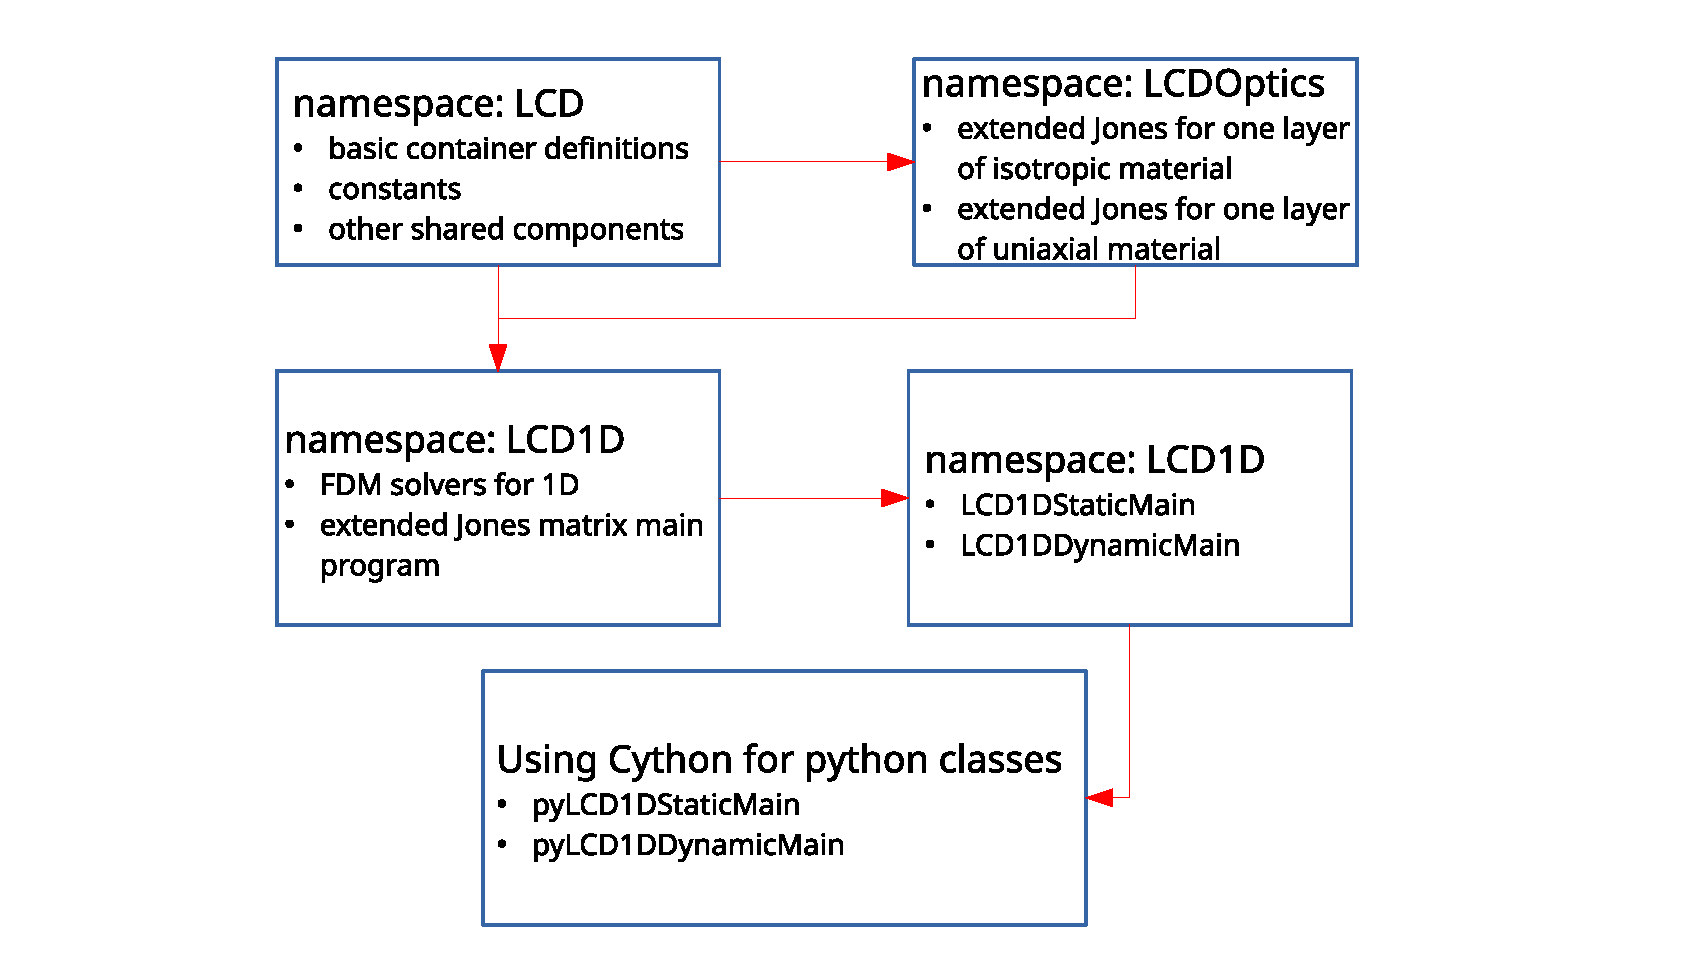
\includegraphics[scale=0.4]{openlcdfdm_structure.eps}
\end{center}
\end{frame}
%\begin{frame}
%\frametitle{Parameters for liquid crystal calculation}
%\begin{itemize}
%\item Elastic constants: $K_{11}$, $K_{22}$ and $K_{33}$
%\item Rotational viscosity: $\gamma$
%\item Dielectric constants:
%	\begin{itemize}
%	\item Dielectric constants parallel to the principal axis $\epsilon_{\parallel}$
%	\item Dielectric constants perpendicular to the principal axis $\epsilon_{\perp}$
%	\end{itemize}
%\item Chirality: It's $q_0=2\pi/p_0$ where $p_0$ is the pitch.
%\item Boudary conditions: The directions of liquird crystal molecule on the surface of LC layer boundary.
%\end{itemize}
%\end{frame}
%\begin{frame}
%\frametitle{Parameters for optical calculation}
%In the optical calculation.
%\begin{itemize}
%\item Isotropic layer:
%	\begin{itemize}
%	\item Layer thickness
%	\item Refractive index distribution 
%	\end{itemize}
%\item Uniaxial layer:
%	\begin{itemize}
%	\item Layer thickness
%	\item Ordinary and extraordinary refractive index distribution.
%	\item Optical axis distribution. (It's not needed if this layer is LC layer.)
%	\end{itemize}
%\end{itemize}
%\end{frame}
\begin{frame}
\frametitle{Demo: V-T curve of twist nematic mode}
\end{frame}
\begin{frame}
\frametitle{Demo: Cono plot of twist nematic mode}
\end{frame}
\begin{frame}
\frametitle{Demo: LC distribution in twist nematic mode}
\end{frame}
\begin{frame}
\frametitle{Future works}
\begin{itemize}
\item Calculate Stokes value to track change of polarization.
\item Implement Berreman 4X4 method
\item Add bixial material support for extended Jones matrix method
\item Bound OpenLCDFDM with FDTD simulation module(ex. meep-FDTD)
\item Move toward 2D and 3D simulation
\end{itemize}
\end{frame}
\begin{frame}
\frametitle{References}
\begin{thebibliography}{0}
\bibitem{Bochi} Optics of Liquid Crystal Display by Pochi Yeh and Claire Gu. ISBN: 0470181761
\bibitem{ShinTson} Fundamentals of Liquid Crystal Devices by Shin-Tson Wu and Deng-Ke Yang. ISBN: 978-0-470-03202-2
\bibitem{modes}{\url{http://www.tftcentral.co.uk/articles/panel_technologies.htm}}
\end{thebibliography}
\end{frame}
%\end{CJK}
\end{document}